\documentclass[mathserif,usenames,professionalfonts,11pt,aspectratio=149]{beamer}

\usepackage{minted}

\newcommand\paper[1]{%
  \begin{textblock*}{\paperwidth}(2pt,0.98\textheight)
    \raggedleft{\tiny #1}\hspace{.5em}
  \end{textblock*}}

\usepackage[utf8]{inputenc}
\usepackage[T1]{fontenc}
\usepackage[protrusion=true,expansion=true]{microtype}
\usepackage[normalem]{ulem} 
\usepackage{amsmath}

%\usepackage[loosequotes,slides]{MinionPro}

\usepackage{bera,berasans,beramono}

\usepackage{tikz}

%%%%%%%%% COLORS

\definecolor{clouds}{HTML}{ECF0F1}

\definecolor{belize}{HTML}{2980B9}
\definecolor{peter}{HTML}{3498DB}

\definecolor{pomegranate}{HTML}{C0392B}

\definecolor{turquoise}{HTML}{1ABC9C}

\definecolor{midnight}{HTML}{2C3E50}

%\setbeamertemplate{background canvas}[vertical shading][top=clouds, bottom=clouds]

\makeatletter
\setbeamertemplate{background canvas}{%
   \ifnum\c@framenumber=1%
      \color{turquoise}\rule{\paperwidth}{\paperheight}
   \fi%
}
\makeatother

\setbeamercolor{normal text}{fg = midnight}
\setbeamercolor{alerted text}{fg = pomegranate}

\setbeamercolor{frametitle}{fg = belize}
\setbeamercolor{framesubtitle}{fg = peter}

\setbeamercolor{title}{fg = white}

\setbeamercolor{structure}{fg = turquoise}

%%%%%%%% FONTS

\setbeamerfont{title}{series=\sffamily}
\setbeamerfont{subtitle}{series=\sffamily}
\setbeamerfont{frametitle}{series=\sffamily}
\setbeamerfont{framesubtitle}{series=\sffamily}


\title[Networks]{A (not so) gentle introduction to networks in ecology}
\author{Timothée Poisot}
\institute[UQAR]{Université du Québec à Rimouski}
\date{\today}

\begin{document}

\frame[plain]{\titlepage}

\section{Introduction}

\begin{frame}{Why should I care about networks?}
   \begin{itemize}
      \item A good way to harness complexity (especially of emergent niche patterns)
      \item A solid mathematical foundation
      \item Elegant algorithms
      \item Visualisations look \emph{awesome}
      \item I'm going to talk about them for, like, two hours\ldots
   \end{itemize}
\end{frame}

\frame[plain]{\centering
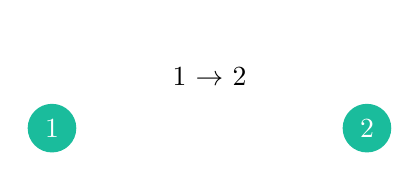
\begin{tikzpicture}[auto, ->, =>stealth', shorten >=1pt, very thick]

\tikzstyle{every node}=[circle, fill=turquoise, draw=none, text=white]
\draw    (0,   0)    node (1) {1}
         (4,  0)  node (2) {2};

\path (1) -> node [draw=none, fill=none, text=black]{1 $\rightarrow$ 2}(2);

\end{tikzpicture}
}

\begin{frame}{What is a network?}{A mathematical approach}
   A \emph{graph} is a \textbf{representation} of a \textbf{set of objects} where some pairs of objects are \textbf{connected} by \textbf{links}.
   \vskip 2em
   Or more formally, $G = (V,E)$, a \emph{graph} $G$ is an ordered pair of \emph{vertices} $V$ linked together by \emph{edges} $E$.
   \vskip 2em
   Each element of $E$ is a two-element subset of $V$.
   \vskip 2em
   The \emph{order} of a graph is $|V|$, and its \emph{size} is $|E|$.
\end{frame}

\begin{frame}{What is a network?}{An example}
   In an omnivory scenario, one top predator $P$ consumes both an intermediate consumer $C$ and a primary producer $R$. The intermediate consumer also consumes the producer.
   \vskip 2em
   \begin{columns}[c]
      \begin{column}{0.5\textwidth}
         This network is specified by
         $$G = \left(\{P, C, R\},\{\{P,C\},\{P,R\},\{C,R\}\}\right) $$
         \vskip 1em
         Or for brevity
         $$G = \left(\{P, C, R\},\{PC,PR,CR\}\right) $$
      \end{column}
      \begin{column}{0.5\textwidth}
         \centering
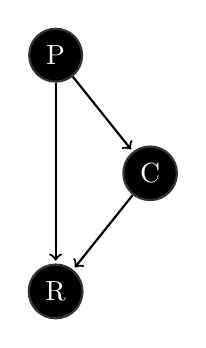
\begin{tikzpicture}[auto, ->, =>stealth', shorten >=1pt, thick]

\tikzstyle{every node}=[circle, fill=black, draw=black!80, text=white]
\draw    (0,   3)    node (pred) {P}
         (1.2, 1.5)  node (cons) {C}
         (0,   0)    node (ress) {R};

\draw (pred) -> (cons);
\draw (pred) -> (ress);
\draw (cons) -> (ress);

\end{tikzpicture}

      \end{column}
   \end{columns}
\end{frame}

\begin{frame}{What is a network?}{The adjacency matrix}
   Networks are often represented by their \textbf{adjacency matrix}.
   \vskip 2em
   The adjacency matrix $\mathbf{A}$ of a graph $G = (V,E)$ has elements $A_{ij}$ with value 1 if there is an edge between the node $V_i$ and the node $V_j$, and 0 otherwise.
\end{frame}

\begin{frame}{What is a network?}{From the graph to the matrix}
   \begin{columns}[c]
      \begin{column}{0.5\textwidth}
         \centering
\begin{tikzpicture}[auto, ->, =>stealth', shorten >=1pt, thick]

\tikzstyle{every node}=[circle, fill=turquoise, draw=none, text=white]
\draw    (0,   3)    node (pred) {P}
         (1.2, 1.5)  node (cons) {C}
         (0,   0)    node (ress) {R};

\draw [thick, draw = wisteria] (pred) -> (ress);
\draw [thick, draw = orange] (cons) -> (ress);
\path [draw = pomegranate] (pred) -> node [draw=none, fill=none, text=black]{A}(cons);
\path [draw = wisteria] (pred) -> node [draw=none, fill=none, text=black]{B}(ress);
\path [draw = orange] (cons) -> node [draw=none, fill=none, text=black]{C}(ress);

\end{tikzpicture}

      \end{column}
      %
      \begin{column}{0.5\textwidth}
         \centering
\begin{tikzpicture}[auto, ->, =>stealth', shorten >=1pt, thick]

\tikzstyle{every node}=[circle, fill=turquoise, draw=none, text=white]
\draw    (1,   4)    node (pred) {P}
         (2,   4)    node (cons) {C}
         (3,   4)    node (ress) {R};

\draw    (0,   3)    node (pred1) {P}
         (0,   2)    node (cons1) {C}
         (0,   1)    node (ress1) {R};

\tikzstyle{every node}=[rectangle, fill=pomegranate, draw=none, text=white]
\draw (2, 3) node (pc) {A};

\tikzstyle{every node}=[rectangle, fill=wisteria, draw=none, text=white]
\draw (3, 3) node (pr) {B};

\tikzstyle{every node}=[rectangle, fill=orange, draw=none, text=white]
\draw (3, 2) node (cr) {C};



\end{tikzpicture}

      \end{column}
   \end{columns}
   ~
   \vskip 3em
   \alert{Exercise}: Re-draw this graph (and the matrix) if $C$ is carnivorous.
\end{frame}

\begin{frame}{What is a network?}{Edge direction}
   Edges can be \emph{directed} (arcs, directed edges) or not. An edge between a vertex and itself (cannibalism) is a \emph{self-loop}.
   \vskip 2em
   In an \textbf{undirected graph}, there are at most $|V|(|V|-1)/2$ edges if there are no \emph{self-loops}.
   \vskip 2em
   In a \textbf{directed graph}, there are at most $|V|(|V|-1)$ edges if there are no \emph{self-loops}.
   \vskip 2em
   \alert{Exercise}: What is the maximal size of a graph of order $n$ if there are self-loops? What is the \emph{minimal} size of the same graph?
\end{frame}

\begin{frame}{What is a network?}{Edge weight}
   Edges in a network can have a \textbf{weight} (for example, the number of contacts between individuals).
   \vskip 2em
   The elements of the adjacency matrix $\mathbf{A}$ can be given \emph{continuous} values.
   \vskip 2em
   It's possible to work both on the \emph{weighted} and \emph{unweighted} properties of a graph. \alert{However}, there are many methods that (as of now) can only be applied to \textbf{undirected, unweighted} networks.
\end{frame}

\begin{frame}{Number of partners}
   The number of vertices \emph{receiving} a link from a focal vertex are called its \textbf{successors}
   \vskip 2em
   The number of vertices \emph{establishing} a link towards a focal vertex are called its \textbf{predecessors}
   \vskip 2em
   The \emph{total} number of edges connected to a focal vertex is this vertex \textbf{degree}
\end{frame}

\begin{frame}{Some remarks on degrees}
   In a graph with $n$ nodes, the degree $k$ of a node $i$ is $k_i = \sum_{j=1}^n A_{ij}$ (\emph{iff} the graph is undirected).
   \vskip 2em
   If there are $m$ edges, there are $2m$ \emph{ends} of edges, with $2m = \sum_{i=1}^nk_i$. In an undirected graph, this is equal to the sum of degrees.
   \vskip 2em
   Thus, $m = \frac{1}{2}\sum_{i=1}^nk_i = \frac{1}{2}\sum_i\sum_j A_{ij}$
   \vskip 2em
   As the mean degree of nodes is simply $c = \frac{1}{n}\sum k_i$, we can write $c = \frac{2m}{n} $.
\end{frame}

\begin{frame}{Some exercises on degrees}
   \alert{Exercise(s)}:
   \vskip 2em
   Using the same approach, find \textbf{the expression of the mean number of predecessors and successors} in a directed graph.
   \vskip 1em
   Discuss the relationship between these two values.
   \vskip 1em
   Is the mean degree different in a directed/undirected network?
\end{frame}

\begin{frame}{Unipartite and bipartite graphs}
   In a \textbf{bipartite} graph, vertices are divided into two distinct sets, with edges established between two vertices from \emph{different} sets.
   \vskip 2em
   This do not happen in \textbf{unipartite} graphs.
   \vskip 2em
   \alert{Exercise}: Discuss the application of bipartite and unipartite networks to ecological systems.
   \vskip 2em
   In a bipartite graph, the adjacency matrix is (formally) called the \textbf{incidence matrix}.
\end{frame}

\begin{frame}{Trees and cycles}

\end{frame}

\section{Paths, shortest paths, and some fun with matrices}

\begin{frame}{Paths}
   A \textbf{path} is a sequence of nodes, so that every consecutive pair of nodes are connected through an edge. You can ``walk'' along edges from the first to the last node along a path.
   \vskip 2em
   The \textbf{length} of a path is the number of \emph{edges} in that path.
   \vskip 2em
   If nodes $i$ and $j$ are connected, then \emph{there is a path of length 1 between them}. If they are connected through $k$, there is \emph{a path of length 2}.
\end{frame}

\begin{frame}{Cycles}
   A \textbf{cycle} is a path from node $i$ to itself, visiting any number of nodes in between.
   \vfill
   \begin{columns}[c]
      \begin{column}{0.5\textwidth}
         \centering
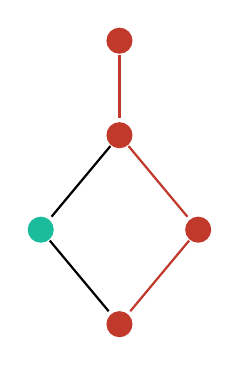
\begin{tikzpicture}[auto, =>stealth', shorten >=1pt, thick]

\tikzstyle{every node}=[circle, fill=turquoise, draw=none, text=white]
\draw     (-1, 1.2) node (in2) {};

\tikzstyle{every node}=[circle, fill=pomegranate, draw=none, text=white]
\draw    (0,   2.4)    node (cons) {}
         (1, 1.2)  node (in1) {}
         (0,   0)    node (ress) {}
         (0,   3.6)  node (pred) {};

\draw [draw = pomegranate] (pred) -- (cons);
\draw [draw = pomegranate] (cons) -- (in1);
\draw (cons) -- (in2);
\draw [draw = pomegranate] (in1) -- (ress);
\draw (in2) -- (ress);

\end{tikzpicture}

      \end{column}
       \begin{column}{0.5\textwidth}
          \centering
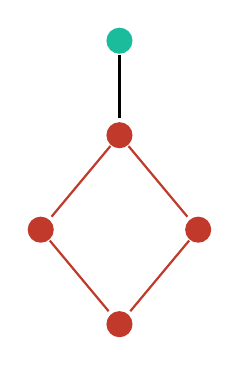
\begin{tikzpicture}[auto, =>stealth', shorten >=1pt, thick]

\tikzstyle{every node}=[circle, fill=turquoise, draw=none, text=white]
\draw    (0,   3.6)  node (pred) {};

\tikzstyle{every node}=[circle, fill=pomegranate, draw=none, text=white]
\draw    (0,   2.4)    node (cons) {}
         (1, 1.2)  node (in1) {}
         (-1, 1.2) node (in2) {}
         (0,   0)    node (ress) {};

\draw (pred) -- (cons);
\draw [draw = pomegranate] (cons) -- (in1);
\draw [draw = pomegranate](cons) -- (in2);
\draw [draw = pomegranate] (in1) -- (ress);
\draw [draw = pomegranate] (in2) -- (ress);

\end{tikzpicture}

       \end{column}
   \end{columns}
\end{frame}

\begin{frame}{Reminder: multiplying matrices}
   \begin{itemize}
      \item Only \emph{square} matrices can be raised to an exponent (\alert{Exercise}: What of bipartite rectangular networks?)
      \item $(\mathbf{AB})_{ij} = \sum_{p=1}^m A_{ik} B_{jk}$
      \item $\mathbf{A}^0 = \mathbf{I}$
      \item $\mathbf{A}^2 = \mathbf{A}\mathbf{A}$
      \item $(r\mathbf{A})^k = r^k\mathbf{A}^k$
      \item $\mathrm{det}(\mathbf{A}^k) = \mathrm{det}(\mathbf{A})^k$ because $\mathrm{det}(\mathbf{A}\mathbf{B}) = \mathrm{det}(\mathbf{A})\mathrm{det}(\mathbf{B})$
   \end{itemize}
\end{frame}

\begin{frame}{Number of paths}
   The number of paths of length $2$ between $i$ and $j$ is given by $$N^{(2)}_{ij} = \sum{k=1}^nA_{ik}A_{kj}$$.
   \vskip 2em
   This is generalized for paths of length $n$ to $$N^{(n)}_{ij} = (\mathbf{A}^n)_{ij} $$.
\end{frame}

\begin{frame}{Number of paths}{A little bit of programming}
   \begin{columns}[c]
      \begin{column}{0.5\textwidth}
         \alert{Exercise}
         \vskip 2em
         Write this undirected network as an adjacency matrix, and calculate the number of paths of length 1, 2, \ldots, between species $1$ and $3$, and between species $1$ and $5$.
         \vskip 2em
         Reminder: $\mathbf{A}\times\mathbf{B}$ = \texttt{A \%*\% B}
      \end{column}
      \begin{column}{0.5\textwidth}
         \centering
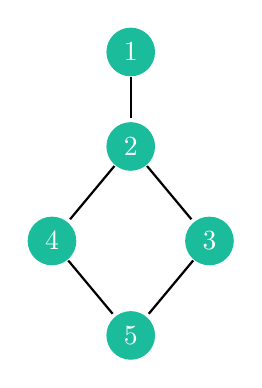
\begin{tikzpicture}[auto, =>stealth', shorten >=1pt, thick]

\tikzstyle{every node}=[circle, fill=turquoise, draw=none, text=white]
\draw     (-1, 1.2) node (in2) {4};
\draw    (0,   2.4)    node (cons) {2}
         (1, 1.2)  node (in1) {3}
         (0,   0)    node (ress) {5}
         (0,   3.6)  node (pred) {1};

\draw (pred) -- (cons);
\draw (cons) -- (in1);
\draw (cons) -- (in2);
\draw (in1) -- (ress);
\draw (in2) -- (ress);

\end{tikzpicture}

      \end{column}
   \end{columns}
\end{frame}

\begin{frame}[fragile]{Number of paths}{A little bit of programming}
   \begin{minted}[linenos]{splus}
matPow = function(A,n)
{
   for(i in c(1:(n-1))) A = A%*%A
   return(A)
}

A = matrix(0, ncol=5, nrow=5)
A[1,2] = A[2,4] = A[2,3] = A[4,5] = A[3,5] = 1
A[2,1] = A[4,2] = A[3,2] = A[5,4] = A[5,3] = 1
for(pathLength in c(0:5)) print(matPow(A, pathLength))
   \end{minted}
   \vskip 2em
   \alert{Exercise}: What happens if the edges are directed (\emph{e.g.} from lower to higher numbers)?
\end{frame}

\begin{frame}{Number of paths}{Find the number of cycles}
   Based on the previous result, we can identify the number of paths of size $n$ from one node to itself, $(\mathbf{A}^n)_{ii}$.
   \vskip 2em
   Because for square matrices, $\mathrm{Tr}(\mathbf{A}) = \sum\mathrm{diag}(\mathbf{A})$, the \emph{total number of cycles of length $n$} is given by $L_{n} = \mathrm{Tr}(\mathbf{A}^n)$.
\end{frame}

\begin{frame}{Identify the shortest path}
   A \textbf{very crude} way to find the shortest path between $i$ and $j$ is to find the \emph{smallest value of $n$} for which $(\mathbf{A}^n)_{ij} > 0$.
   \vskip 2em
   The shortest path is called the \textbf{geodesic} path.
   \vskip 2em
   This method in inefficient, and modern software implements much better search strategies.
\end{frame}

\begin{frame}{Other remarkable paths}
   An \textbf{Eulerian path} visits each \emph{edge} once. The graph is Eulerian (unicursal) if this path is a cycle, and semi-Eulerian (traversable) if not.
   \vskip 2em
   A \textbf{Hamiltonian path} visits each \emph{node} once. A graph with a Hamiltonian path is traceable.
   \vskip 2em
   \alert{Exercise}: Prove that for a complete undirected graph with $n$ nodes, there are $(n-1)!/2$ Hamiltonian paths.

\end{frame}

\section{A little bit of ecology}

\begin{frame}{Where is the ecology in all that?}
   \begin{description}
      \item[graph] The whole community, \emph{i.e.} the populations and their interactions
      \item[vertices] The composition of the community (species present)
      \item[edges] The interactions between the populations
   \end{description}
\end{frame}

\begin{frame}{Where is the ecology in all that?}{Example of ``networkable'' systems}
   \begin{itemize}
      \item Trophic systems
      \item Plant--pollinators
      \item Hosts--parasites
      \item Mutualism
      \item Social interactions
   \end{itemize}
   \vskip 2em
   Any system in which the \textbf{same ecological interaction} happens several time in a community can (should) be studied using network theory
\end{frame}

\section{Representing networks}

\section{Network-level properties}

\begin{frame}{Connectance}
   Connectance is the \emph{proportion of possible interactions realized} (also called the density $\rho$ in graph theory)
   \vskip 2em
   The order of an ecological network is usually called $S$, and its size $L$
   \vskip 2em
   Ecologists often define connectance as $Co = L/S^2$.
   \vskip 2em
   \alert{Exercise}: What do you think of this definition based on results about the maximal order of a graph or size $S$?
\end{frame}

\section{Vertex-level properties}

\begin{frame}{Number of partners}
   The number of (\emph{e.g.}) preys of a predator is its \textbf{generality} (number of successors)
   \vskip 2em
   The number of (\emph{e.g.}) predators of a prey is its \textbf{vulnerability} (number of predecessors)
\end{frame}

\begin{frame}[fragile]{Number of partners}
   \begin{minted}[linenos]{splus}
      web = read.table('web.dat')
      generality = rowSums(web)
      vulnerability = colSums(web)
      degree = generality + vulnerability
   \end{minted}
\end{frame}

\section{Generating networks}

\begin{frame}{Null models}{The ecological use}
   Even just \emph{by chance}, networks will have statistical properties. The truth is in the residuals.
   \vskip 2em
   \textbf{Null models} allow to disentangle the random and non-random properties of networks.
   \vskip 2em
   Example of a question: is a given network more or less nested than expected by chance?
\end{frame}

\begin{frame}[fragile]{Null models}{WTF is nestedness?}
   \begin{columns}[c]
      \begin{column}{0.5\textwidth}
         In a \emph{nested} network, \alert{a species with a degree $d_i$ interacts with a subset of the species with a degree $d_j$ so that $d_j>d_i$}.
         \vskip 1em
         The more this is true, the more a network is nested.
       \end{column}
      \begin{column}{0.5\textwidth}
         \centering
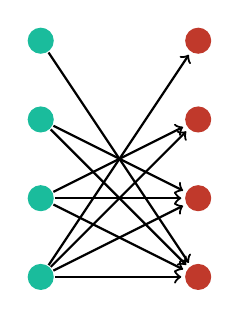
\begin{tikzpicture}[auto, ->, =>stealth', shorten >=1pt, thick]

\tikzstyle{every node}=[circle, fill=turquoise, draw=none, text=white]
\draw    (0,   0)    node (p0) {}
         (0,   1)    node (p1) {}
         (0,   2)    node (p2) {}
         (0,   3)    node (p3) {};

\tikzstyle{every node}=[circle, fill=pomegranate, draw=none, text=white]
\draw    (2,   0)    node (f0) {}
         (2,   1)    node (f1) {}
         (2,   2)    node (f2) {}
         (2,   3)    node (f3) {};

\draw (p0) -> (f0);
\draw (p0) -> (f1);
\draw (p0) -> (f2);
\draw (p0) -> (f3);

\draw (p1) -> (f0);
\draw (p1) -> (f1);
\draw (p1) -> (f2);

\draw (p2) -> (f0);
\draw (p2) -> (f1);

\draw (p3) -> (f0);



\end{tikzpicture}

      \end{column}
   \end{columns}
   \vskip 2em
   \begin{minted}[linenos]{splus}
library(vegan)
web = read.table('matrix.txt')
nestednodf(web)
   \end{minted}
\end{frame}

\begin{frame}{Null models}{The basic approach}
   We want to simulate \emph{pseudo-random} networks that reproduce \emph{some} features of the empirical (observed) network.
   \vskip 2em
   For any empirically measured property $X$, we will have a distribution of $\mathcal{X}$.
   \vskip 2em
   We might want to test that $\sum(X-\mathcal{X})/n = 0$, \emph{i.e.} the observed property is not significantly different from the random expectation.
\end{frame}

\begin{frame}{Null models}{Controlling for mean degree}
   This is formally called a \emph{Erd\"os--Renyi graph}. Each pair of nodes has a probability $\rho$ of being connected.
   \vskip 2em
   \alert{Exercise:} write a function in R filling a matrix with 0 and 1 at random.
\end{frame}

\begin{frame}{Null models}{Controlling for node degree}
   We want each node to receive and establish interactions (almost) as in the original network.
   \vskip 1em
   $$P(i\rightarrow j) = \frac{1}{2}\left(\frac{g_i}{d_i}+\frac{v_j}{d_j}\right)$$
   \vskip 2em
   \alert{Exercise:} Using operations on matrices, write a function to generate a random network in R, conserving either the connectance, or the degrees.
\end{frame}

\begin{frame}{The niche model of food webs}
   \begin{columns}[c]
      \begin{column}{0.5\textwidth}
         \begin{itemize}
            \item Small stuff produces stuff
            \item Large stuff east smaller stuff
            \item Sometimes that's not entirely true
         \end{itemize}
      \end{column}
      \begin{column}{0.5\textwidth}
      \end{column}
   \end{columns}
\end{frame}

\end{document}
